% !TEX root = ../main.tex

\chapter{Methodology}
\label{chapter:Methodology}
We identify two main challenges with the single observation sparse reward setup. \\
\section{Curse of Dimensionality}
As introduces in \ref{COD}, the evidence for a model scales approximately inversly proportinal to the exponent of the dimension on which it acts. In MDPs, the 
actor $\pi$ acts on the observation space and returns an action from the action space. A probabalistic actor defines a probability distribution on the set 
of actions $\mathcal{A} \in \mathcal{R}^m$ and observations $\mathcal{O} \in \mathcal{R}^n$ as $\pi(a|o) = \frac{p(a,o)}{p(o)}$. 
Thus the dimension on which the actor acts on, is $n \times m$ with $\pi:\mathcal{R}^m \times \mathcal{R}^n \rightarrow \mathcal{R}$.\\
Similarely, the critic $Q$ usually defines a function on $\mathcal{A}$ and $\mathcal{O}$ to the comulative discounted expected value 
$Q:\mathcal{R}^m \times \mathcal{R}^n \rightarrow \mathcal{R}$, while TQC defines the critic as a quantile distribution: 
$Q:\mathcal{R}^m \times \mathcal{R}^n \rightarrow \mathcal{R}^k$ with $k$ quantiles.\\
We have shown in \ref{POMDP}, that in a POMDP, the observation space grows linear in time. Together with the result from \ref{COD} we conclude, that we have 
exponentially less evidence with sequence length $T$ for our model in the POMDP setting.\\
To counter this problem, we want to get rid of the time dependency of the belief state. To do this, 
we make the observation, that our case with the single observation at the beginning is a special case of a POMDP. Usually, 
we need to know all previous obervsations, as they can give us additional information about the believe state. However, as we don't have subsequent information 
after the initial observation, the only knowledge we have to include to calculate our believe state are the actions, that the policy took. As introduced in \ref{pomdp_bayes}, the optimal believe state 
update in the general POMDP case using bayes theorem is given by:
\begin{equation}
    b_{t+1}(s') = \frac{\mathcal{Z}(s', o_{t+1}) \sum_{s \in \mathcal{S}} \mathcal{T}(s, a_t, s') b_t(s)}{\sum_{s'' \in \mathcal{S}} \mathcal{Z}(a_t, s'', o_{t+1}) \sum_{s \in \mathcal{S}} \mathcal{T}(s, a_t, s') b_t(s)}
\end{equation}
. In our case, we can rewrite this as:
\begin{equation}
    b_{t+1}(s') = \frac{\mathcal{Z}(s', o_{0}) \sum_{s \in \mathcal{S}} \mathcal{T}(s, a_t, s') b_t(s)}{\sum_{s'' \in \mathcal{S}} \mathcal{Z}(s'', o_{0}) \sum_{s \in \mathcal{S}} \mathcal{T}(s, a_t, s') b_t(s)}
\end{equation}
. $\mathcal{Z}(s'', o_{0})$ is constant for $t>0$, so we get:
\begin{equation}
    b_{t+1}(s') \propto \sum_{s \in \mathcal{S}} \mathcal{T}(s, a_t, s') b_t(s) \quad | t > 0
\end{equation}
\begin{equation*}
    b_{0}(s') \propto \mathcal{Z}(s', o_{0})
\end{equation*}
. If we assume a deterministic policy $\pi(a|b) \rightarrow a_{\pi}(b)$, the update step can be written as:
\begin{equation}
    b_{t+1}(s') \propto \sum_{s \in \mathcal{S}} \mathcal{T}(s, a_{\pi}(b_t), s') b_t(s)
\end{equation}
. By using this update step recursively until we get to $b_{0}$, we see, that the believe state at time $t$ only depends on the initial observation $o_0$
the transition probability $\mathcal{T}$ and the number of recursion steps $t$. Using this insight, we can rewrite the belief state at timestep $t$ like:
\begin{equation}
    b_{t+1}(s') \propto \mathcal{Z}(s_0, o_{0}) \mathcal{T}(s_0, s', t)_{\pi}
\end{equation}
, where $\mathcal{T}(s_0, s', t)_{\pi}$ indicates that the normalized transition function depends on the timestep $t$ and policy $\pi$.\\
With this formulation, we can rewrite the policy 

\begin{equation}
    \pi(a|b) : \mathcal{R}^m \times \mathcal{R}^{n T} = \pi(a|o_0, t): \mathcal{R}^m \times \mathcal{R}^{n} \times 1.
\end{equation}
We call this a strong inductive belief state bias for the single observatino POMDP, as it forces the assumption of a deterministic and constant policy $\pi$. 
In our method, we implement a weak inductive bias, which is motivated by this observation: We use transformer encoder type architecture, which inputs are 
the repeated initial observation plus a positional encoding. We then use a single pass through the network, which means it does not work autoregressively and 
relies less on former actions to determin action at time point $t$. We test this hypothesis by using baselines that have the strong inductive bias, as well as 
using the transformer in autoregressive mode. \\

\section{Update Error}
As we only have a single observation, our model has to learn the dynamics of the MDP in order to predict the reward signal at time point $t > 1$. In \cite{NEURIPS2020_b5c01503} 
it has been shown, that learning a transition model for an mdp has a quadratic error bound in $\gamma$ thus we expect quadratic error with the length of the horizon. 
However, we identify that this challange also grants us a unique improvement over previous actor critic methods. By predicting whole sequences of actions at once, 
we show that we can eliminate errors in the update step of the actor.\\
All parametrized actor critic mehtods are technically speaking off policy, as the critic value is bootstrapped with former estimates. Once the actor is updated, the 
critic target moved, on which the actor was updated. Intuitively, when the policy is changed to choose a different action at time point $t$, it might also change 
the policy to choose different actions at 
all subsequent time points, which changes the value function. This leads to unstable update behaviour and is the main reason, why algorithms like PPO try to 
make sure, that changes to the policy are limited. This update instability is specifically challenging in our one observation environment, as the policy does not 
get updates of the state of the environment it is currently in. \\
Formally, let's define the objective function $J(\phi, \theta(\phi)) = \mathbb{E}_{\tau \propto \pi(\phi)}\left[Q_{\theta(\phi)}\right]$ for actor critic methods as the function we whish to optimize to learn the optimal policy. 
$Q_{\theta(\phi_i)}$ indicates the $Q$ function for policy $\pi_{\phi_{i}}$ parametrized by parameters 
$\theta(\phi_i)$. For example, DDPGs policy update rule \ref{AC_general_update} is written as:
\begin{equation}
    \nabla_{\phi} J(\phi, Q(\theta(\phi))) = \mathbb{E}_{\tau \sim p(\tau | \pi_{\phi})} \left[\nabla_{\phi} \log \pi(a_t|s_t;\phi) Q_{\theta, \pi_\phi}(a_t, s_t) \right].
\end{equation}
. Note that generally, we do not have access to $\theta(\phi)$, but only an approximation given the limited data we have collected. Let us denote the actual 
$Q$ function we have as $Q(\theta(\phi) + \epsilon)$, where $\epsilon$ indicates an error between the optimal parameters and the actual parameters.
Let us now for simplicity assume, that $\phi$ and $\theta$ are one dimensional. A generalisation to n dimensions is straight forward, but less readable. We want 
to estimate the update error to $\pi$ from the objective $J$. The proper derivative is given by:
\begin{equation}
    \nabla_{\phi} J(\phi, \theta(\phi)) = \frac{J(\phi + \delta \phi, \theta(\phi + \delta \phi)) - J(\phi, \theta(\phi))}{\delta \phi} + \mathcal{O}(\delta)
\end{equation}
with 
\begin{equation}
    J(\phi + \delta \phi, \theta(\phi + \delta \phi)) = J(\phi, \theta(\phi)) + \left[ 
        \frac{\partial J}{\partial \phi} + \frac{\partial J}{\partial \theta} \frac{\partial \theta}{\partial \phi}
    \right] \delta \phi  + \mathcal{O}(\delta^2)
\end{equation}
, where we used the chain rule and taylor's theorem. 
We can express this in terms of the parametrs $\theta(\phi) + \epsilon$:
\begin{equation}
    \nabla_{\phi} J(\phi, \theta(\phi)) = \nabla_{\phi} J(\phi, \theta(\phi) + \epsilon) - \nabla_{\phi} J(\phi, \theta(\phi)) + \nabla_{\phi} J(\phi, \theta(\phi))
\end{equation}
\begin{equation*}
    = \nabla_{\phi} J(\phi, \theta(\phi)) + \epsilon_{\nabla_{\theta}}
\end{equation*}
. Note that $\nabla_{\phi} J(\phi, \theta(\phi) + \epsilon)$ is not a properly defined derivative. To rigorously capture the stochastic dependence of $\theta(\phi)$ 
given a dataset $\mathcal{D}^n$ with $n$ transitions, 
we could formulate $\theta(\phi)|\mathcal{D}_n$ as n boundary conditions. Together with a suitable regularizor, we can then find $\theta_{\epsilon, n}(\phi)$. We omit 
this step, as we are only interested in the fact that there is an error, not the exact value of it.\\
In actor critic policy updates, $\theta$ is assumed a constant, thus the actor derivative 
$\widetilde{\nabla}_\phi J$ of $J$ is given by:
\begin{equation}
    \widetilde{\nabla}_\phi J(\phi, \theta) =  \frac{J(\phi + \delta \phi, \theta) - J(\phi, \theta)}{\delta \phi} + \mathcal{O}(\delta)
\end{equation}
. 
Again using $\theta(\phi) + \epsilon$ we get:
\begin{equation}
    \widetilde{\nabla}_\phi J(\phi, \theta + \epsilon) = \widetilde{\nabla}_\phi J(\phi, \theta) + \epsilon_{\widetilde{\nabla}_{\theta}}
\end{equation}
We can now derive the update error in the actor update:
\begin{equation}
    \nabla_{\phi} J(\phi, \theta(\phi)) - \widetilde{\nabla}_\phi J(\phi, \theta) = \nabla_{\phi} J(\phi, \theta(\phi) + \epsilon) - \epsilon_{\nabla_{\theta}} - \widetilde{\nabla}_\phi J(\phi, \theta(\phi) + \epsilon) + \epsilon_{\widetilde{\nabla}_{\theta}}
\end{equation}
\begin{equation*}
    = \epsilon_{\widetilde{\nabla}_{\theta}} - \epsilon_{\nabla_{\theta}} + \frac{\partial J}{\partial \theta} \frac{\partial \theta}{\partial \phi}
\end{equation*}
. We will call $\epsilon_{\widetilde{\nabla}_{\theta}} - \epsilon_{\nabla_{\theta}}$ the  \textbf{function approximator error}. \\
Recall that $J(\phi, \theta(\phi)) = \mathbb{E}_{\tau \propto \pi(\phi)}\left[Q_{\theta(\phi)}\right]$, so the partial derivative $\frac{\partial J}{\partial \theta} = 1$, 
as the expectation commutes with the derivative. This leaves us with estimating $\delta \frac{\partial \theta}{\partial \phi}$. Again using taylor's theorem, we get 
\begin{equation}
    \label{dist_shift_error}
    \delta \frac{\partial \theta}{\partial \phi} = \theta(\phi + \delta) - \theta(\phi) + \mathcal{O}(\delta).
\end{equation}
We will call this error the \textbf{distribution shift error}.\\
While this derivation assumes direct policy gradient to update the actor, other actor critic policy update methods like the minimisation of a KL divergence as 
proposed is SAC will have similar terms (\cite{SAC}, equation 13).

\subsection{Distribution Shift Error}
From \ref{dist_shift_error} we see, that the error of the update of $\pi$ is proportinal to the change in the 
expected value of $r(\pi)$.\\ 

Eher in function approximator bereich
In the paper "Trust Region Policy Optimization" \cite{TRPO} the authors derive a lower bound on the policy improvement given the KL divergence between the new policy $\tilde{\pi}$ 
at step $i+1$ and the old policy at step $i$ as. Let $\rho_{\pi}(s)$ be the occupancy measure of state $s$ given policy 
$\pi$ let $L_{\pi}(\tilde{\pi}) = J(\pi) + \sum_s \rho_{\pi}(s) \sum_a \tild{\pi}(a|s) A_\pi(s,a)$ 
be the expected discounted reward of policy $\tild{\pi}$ given the occupance measure of policy $\pi$ with the advatage function $A$. It can be shown, that 
\begin{equation}
    J(\tilde{\pi}) \geq L_\pi(\tilde{\pi}) - C D_{\max} \mathrm{KL}(\pi, \tilde{\pi}),
\end{equation}
where $C = 4\epsilon\gamma/(1-\gamma)^2$ and $\epsilon = \max_{s,a} |A_\pi(s,a)|$. Although not directly comparable, this falls in line with our approximation of the update error, as 
the negative term on the right side of the inequality scales linear with the KL divergence between the old policy $\pi$ and the new policy $\tilde{\pi}$. \\
The point of this analysis is to show, that inherently actor critic policies make policy update errors and tend to overestimate value functions, 
which makes using data collected from earlier policies challenging. We have discussed one way to counter this problem in our section about TQC \ref{section:TQC}, 
where the overestimation bias was derived differently, but the methods main focus was on introducing a parameter, with which this overestimation can be controlled. 
While it shows good results in practice, solving this problem by introducing a mechanism that can use a hyper parameter to emperically counter the update error 
entails the reliance on hyper parameter tuning. \\


In our aproach, we want to decouple the critic from the actor to set the distribution shift error to zero. To do so, let's see where the difference between 
$\theta(\phi)$ and $\theta(\phi + \delta)$ comes from. Recall when we write $\theta(\phi)$ we mean $Q_{\theta}(a,s|\pi_{\phi})$:
\begin{equation*}
    Q_{\theta}(a,s|\pi_{\phi}) = \mathbb{E}_{(a_t \propto \pi_{\phi}(s_t), s_t \propto T(s_{t-1}, a_{t-1}, s_t))|a_0=a, s_0=s}\left[\sum_t \gamma^t r(a_t, s_t)\right]
\end{equation*}
from that we get
\begin{equation}
    Q_{\theta }(a,s|\pi_{\phi + \delta}) - Q_{\theta}(a,s|\pi_{\phi}) != 0 \text{ if } \pi_{\phi + \delta}(a|s) != \pi_{\phi}(a|s)
\end{equation}
except for degenerate cases. We propose a whole sequence actor critic, where given an observation, the actor proposes the whole sequence of actions it will 
take and the critic uses the whole sequence of actions to predict all rewards. The new $Q_{\text{whole sequence}}$ is thus defined on an observation and a 
sequence of actions: 
\begin{equation}
    (a_0, ..., a_T) \propto \pi_{\text{whole sequence}}(a_0, ..., a_t|s)
\end{equation}
\begin{equation*}
    Q_{\text{whole sequence}}(t, s, a_0, ..., a_T) = \mathbb{E}_{s_t \propto T(s_{t-1}, a_{t-1}, s_t) | s_0=s}\left[r(a_t, s_t)\right]
\end{equation*}
Note, that as there is no dependency of $Q$ on $\pi$, the distribution shift error \ref{dist_shift_error} is zero. The downside of this approach is, that the 
critic has to predict the MDP, to predict the correct reward after the action sequence $a_{0, ... t}$. While predicting an MDP entailes a quadratic error in 
$\gamma$, it has been shown to be useful for example as a regularizor in \ref{GAIL_POMDP} and as a proxy loss in \ref{MUESLI}. Note, that our 
formulation does not train the policy to predict the exact observations at time step t, but rather it is trained to only predict the expected reward. 
In our discussion of \ref{GAIL_POMDPS} we stated, that predicting exact observations is unnecessarly hard and not optimally aligned with the actual objective. 
Our whole sequence critic only has to learn a value equvialent MDP \ref{https://arxiv.org/abs/2011.03506}.\\
While our approach is generally applicable in all MDPs, it is specifically usefull in our environment with only one observation, as in this setup, we can't do 
better then to predict all actions and the reward $T$ steps into the future, as we don't get any other signal.\\ \\

\subsection{Function Approximation Error}
1. Recall only n boundary conditions -> theta + epsilon. 
2. Intuitively we know Q value only for trj that we saw and approximate Q value for new trajectory. 
3. Decouple Actor from critic: update actor w.r.t. sampled trajectories. For example, only successful trjs. 
4. Improve actor performance by using critic in inference time to sample new actions. 
5. Thus the name: active critic.

\subsection{Average Actions Problem}
In imitation case: what if two trj. lead to success and are both found by the critic? Average trj. between those two probably not correct. Inverse plan to 
disambugate trjs. in inference time, always start with zero plan.

\subsection{Inference Time optimisation}
Multiple options what to optimize: Actions, Actor, Plan. Assumptions: smallest state space is most sample efficient. Optimize on actions is most general.

The other identified error signal in the update step for our policy comes from the fact that we use a function approximator for the $Q$ value. From temporal 
difference learning we get the update signal for our $Q$ function as derived in \ref{Q-ValueTD}:
\begin{equation}
    \delta_t = r_t + \gamma Q_{\theta}(s_{t+1}, a_{t+1}\propto \pi_{\phi}) - Q_{\theta}(s_{t}, a_{t} \propto \pi_{\phi})
\end{equation}
. If we change $\pi_{\phi}$, 

Instead use TQC error bound (https://arxiv.org/pdf/1502.05477.pdf) (8). 
Say, that ising old data has high KL divergence and not using old data means less data efficient. also, mention quadratic error from imitation and 
distribution shift (high KL divergence) between current policy and expert policy.
KL constrain only for one step update, as rho must be reevaluated -> not data efficient. 
Active Critic with whole sequence prediction

Value equivalent MDP, usually only few steps, because compounding errors, but in our case, we only have one observation, so we can know all actions from observation 0. 

Actor is learned to minimize quadratic error of trajectories, what if two different trj. but middle is not good? inverse plan

Abbildung whole algorithm
Meta code whole algorithm.


The SAC update rule in \ref{SAC_update_rule}. We will restate the DDPG update rule, to 
\ref{NEURIPS2020_b5c01503}, theorem 1, states:

We can see this with the example of the SAC objective \ref{sac_pol_obj}, but the argument holds in general for actor critic methods.  
\begin{equation}
    \label{AC_general_update}
    \nabla_{\phi} J(\phi) = \mathbb{E}_{\tau \sim p(\tau | \pi_{\phi})} \left[\nabla_{\phi} \log \pi(a_t|s_t;\phi) Q_{\theta}(a_t, s_t) \right]
\end{equation}




First, frame the curse of dim. for this setup
Make the observation, that with deterministic policy and sequence encoding, principially the wohle informationmoght be in one observation.
State that we call this strong inductive bias. 
Give the policy this inherent strucuter, but the ability to see what it did before
AC - actor with positional encoding and not autoregressive
Improve performacne? Lets revisit (SAC).
Variacne in estimate because 
-overestimation (TQC)
-Iteration Error

New Approach: AC
No overestimation, No Iteration Error
Stabe update to the actor by Imitation setup from newly found correct trajectories
explain L2-problem and solution
Critic learns implicit believe representation for value equvialent MDPs, directly task oriented. (Equivalence of MDPs) (https://proceedings.neurips.cc/paper/2020/file/3bb585ea00014b0e3ebe4c6dd165a358-Paper.pdf)
State whole algorithm.

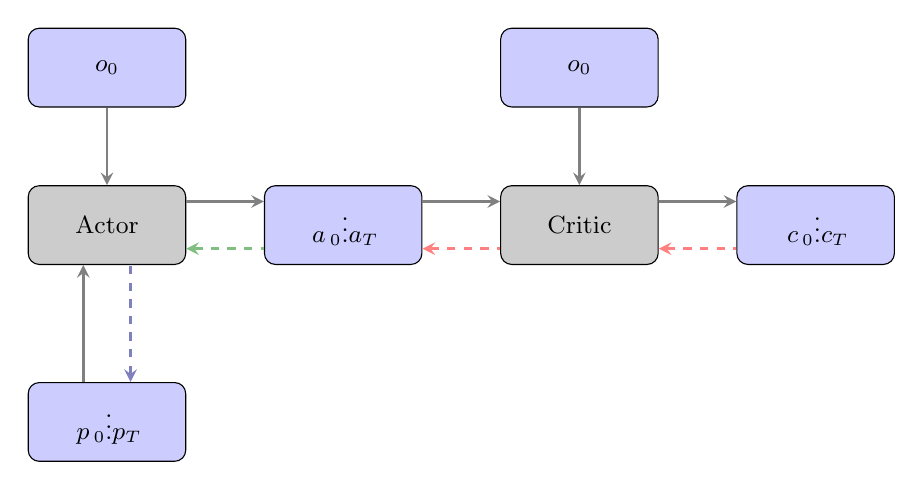
\begin{tikzpicture}[>=stealth,font=\small]
    
    % Define node styles
    \tikzstyle{observation_block_1} = [draw, rounded corners, fill=blue!20, minimum width=2cm, minimum height=1cm, text centered]
    \tikzstyle{actor_block} = [draw, rounded corners, fill=black!20, minimum width=2cm, minimum height=1cm, text centered]
    \tikzstyle{critic_block} = [draw, rounded corners, fill=black!20, minimum width=2cm, minimum height=1cm, text centered]
    \tikzstyle{actions_block} = [draw, rounded corners, fill=blue!20, minimum width=2cm, minimum height=1cm, text centered]
    \tikzstyle{critic_reward_block} = [draw, rounded corners, fill=blue!20, minimum width=2cm, minimum height=1cm, text centered]
    \tikzstyle{observation_block_2} = [draw, rounded corners, fill=blue!20, minimum width=2cm, minimum height=1cm, text centered]
    \tikzstyle{plan_block} = [draw, rounded corners, fill=blue!20, minimum width=2cm, minimum height=1cm, text centered]
    
    % Draw nodes
    \node [actor_block] (actor) {Actor};
    \node [observation_block_1, above of=actor, yshift=1cm] (observations_vector_1) {$o_0$};
    \node [plan_block, below of=actor, yshift=-1.5cm] (plans_vector) {$\begin{matrix}p_0\\ \vdots\\ p_T\end{matrix}$};
    \node [actions_block, right of=actor, xshift=2cm] (actions_vector) {$\begin{matrix}a_0\\ \vdots\\ a_T\end{matrix}$};
    \node [critic_block, right of=actions_vector, xshift=2cm] (critic) {Critic};
    \node [observation_block_2, above of=critic, yshift=1cm] (observations_vector_2) {$o_0$};

    \node [critic_reward_block, right of=critic, xshift=2cm] (critic_reward_vector) {$\begin{matrix}c_0\\ \vdots\\ c_T\end{matrix}$};

    % Draw arrows
    \draw [->, black!50, line width=1pt] (actor.east) ++(0, +0.3cm) --node[midway, above] {} (actions_vector.west |- 0,+0.3cm);
    \draw [<-, green!50!black!50, line width=1pt, dashed] (actor.east) ++(0, -0.3cm) --node[midway, above] {} (actions_vector.west |- 0,-0.3cm);

    \draw [<-, blue!50!black!50, line width=1pt, dashed] (plans_vector.north) ++(+0.3cm, 0) --node[midway, above] {} (actor.south -| 0.3cm,0);
    \draw [->, black!50, line width=1pt] (plans_vector.north) ++(-0.3cm, 0) --node[midway, above] {} (actor.south -| -0.3cm,0);

    \draw [->, black!50, line width=1pt] (observations_vector_1)  --node[midway, above] {} (actor);
    \draw [->, black!50, line width=1pt] (observations_vector_2)  --node[midway, above] {} (critic);


    \draw [->, black!50, line width=1pt] (actions_vector.east) ++(0, +0.3cm) --node[midway, above] {} (critic.west |- 0,+0.3cm);
    \draw [<-, red!50, line width=1pt, dashed] (actions_vector.east) ++(0, -0.3cm) --node[midway, above] {} (critic.west |- 0,-0.3cm);

    \draw [->, black!50, line width=1pt] (critic.east) ++(0, +0.3cm) --node[midway, above] {} (critic_reward_vector.west |- 0,+0.3cm);
    \draw [<-, red!50, line width=1pt, dashed] (critic.east) ++(0, -0.3cm) --node[midway, above] {} (critic_reward_vector.west |- 0,-0.3cm);

    %\draw [->, double] (actions_vector) -- node[midway, above] {} (critic);
    %draw [->, double] (critic) -- ++(-0.1cm) node[midway, above] {} (vector2);
    %\draw [<-, double] (critic) -- ++(-0,1cm) node[midway, above] {} (vector2);
\end{tikzpicture}

